\documentclass[12pt,a4paper,oneside]{article}

\usepackage{fullpage}
\usepackage{url}

% allows including pictures
\usepackage{graphicx}

% for code-snippets
\usepackage{listingsutf8}
\usepackage{color}
\usepackage{enumitem}

%% LISTINGS
\lstset{
	basicstyle       = \ttfamily\footnotesize,			% the size of the fonts that are used for the code
	identifierstyle  = \color[rgb]{0,0,0},				% style for identifiers
	keywordstyle     = \color[rgb]{0,0,1},				% lvl 1 is real keywords
	keywordstyle     = {[2]\color[rgb]{.6,0,0.3}},		% lvl 2 is types
	keywordstyle     = {[3]\color[rgb]{0,.6,0}},		% lvl 3 is something else entirely
	keywordstyle     = {[4]\textbf},					% lvl 4 are special functions
    commentstyle     = \color[rgb]{0.133,0.545,0.133},
    stringstyle      = \color[rgb]{0.627,0.126,0.941},
    showstringspaces = false,
	tabsize          = 2,
	backgroundcolor  = \color{white},
	literate         = {Ö}{{\"O}}1{Ä}{{\"A}}1{Ü}{{\"U}}1{ß}{{\ss}}2{ü}{{\"u}}1{ä}{{\"a}}1{ö}{{\"o}}1	% umlaute
}

\lstset{language=C++}

\newcommand{\cpp}[1]{\lstinline[language=C++]{#1}}
\newcommand{\java}[1]{\lstinline[language=Java]{#1}}

\begin{document}
	% document data
	\title{Project in Software Engineering \& Internet Computing }
	\author{Fabian Gruber, 0726905}

	\maketitle

\section*{Introduction}
	During my project in Software Engineering \& Internet Computing I've worked on cleaning up and improving the codebase of the
	Cacao Java Virtual Machine.
	Chapter \ref{new_apis} describes APIs in Cacao that are either new or changed,
	chapter \ref{repair} gives an overview of fixed bugs and
	chapter \ref{cleanup} sums up the code cleanup done during the project.

\section{New or refactored APIs}
\label{new_apis}

\subsection{New UTF8/UTF16 decoder/encoder}
	The Java Virtual Machine uses a modified UTF-8 encoding\cite{jvmutf8} for string content in class files,
	the Cacao VM also uses this encoding for internally used strings at runtime.
	The Java language on the other hand uses UTF-16 encoded strings.
	Previously Cacao contained three different functions for validating and decoding UTF-8 content to UTF-16
	and three more for the reverse direction.
	Every one of these duplicated the string encoding logic for a slightly different task.
	The various debug routines for displaying strings also contained a lot of boilerplate copies of string traversal code.
	I have introduced two new template functions, \cpp{utf8::transform} and \cpp{utf16::transform}, that have replaced all the old decoding functions.

	A major source of complexity in the old codebase was that it intermingled the process of traversing the characters of an
	encoded string, performing computations on those characters and error handling.
	The two new decoders separate these concerns, each represents just a traversal of a string that invokes
	callbacks passed in as a template parameter. This is similar to how SAX XML parsers operate.
	A nice side of effect of this model is that it is much easier to combine different processing steps.
	Previously validating a UTF-8 string and computing its hash value and size was done in multiple traversals,
	this is now achieved in one pass requiring fewer lines of code.

\clearpage
\subsubsection{UTF-8 API}
	The function for operating on UTF-8 strings is
		\begin{lstlisting}
	template<typename Iterator, typename Visitor>
	typename Visitor::ReturnType utf8::transform(Iterator begin,
	                                             Iterator end, 
	                                             Visitor  v);
		\end{lstlisting}

	\cpp{begin} and \cpp{end} are STL style iterators containing the UTF-8 encoded string,
	ususally they are just a regular \cpp{const char*}.
	The \cpp{Visitor} type contains the callbacks invoked during decoding, it must conform to the following interface:
		\begin{lstlisting}
	struct Visitor {
		typedef ... ReturnType;     // the result of traversing the string

		void utf8(uint8_t);         // called for every valid UTF-8 byte
		void utf16(uint16_t);       // called for every valid UTF-16 codepoint

		ReturnType finish();        // called on success

		ErrorAction error_action(); // called when an error is encountered
		ReturnType  abort();        // called if ErrorAction is ABORT_ON_ERROR
	};
		\end{lstlisting}
	\vspace*{5pt}
	where \cpp{ErrorAction} is defined as follows
		\begin{lstlisting}
	enum ErrorAction {
		IGNORE_ERRORS,    // Invalid input leads to undefined behaviour.

		ABORT_ON_ERROR    // The decoding is aborted an the result of
		                  // Visitor::abort() is returned.
	};
		\end{lstlisting}

	During decoding the visitors methods \cpp{utf8()} and \cpp{utf16()} are called,
	they should contain the main processing logic.
	If no error occurred the final result is computed via \cpp{Visitor::finish()}.

	When an error is encountered during decoding the visitor is queried how it wants to react 
	via its \cpp{error_action()} method.
	It can then decide to,
	\begin{enumerate}[label=\alph*)]
		\item errors lead to undefined behaviour.
		\item abort and return the result of \cpp{abort()}.
	\end{enumerate}

	The class \cpp{utf8::VisitorBase} can be used to reduce the amount of boilerplate required in writing a visitor,
	it contains a dummy implementation of every method required of a visitor type.
	When implementing you only override the methods you actually use.

\subsubsection{UTF-16 API}
	The function for operating on UTF-8 strings is
		\begin{lstlisting}
	template<typename Iterator, typename Visitor>
	typename Visitor::ReturnType utf16::transform(Iterator begin,
	                                              Iterator end, 
	                                              Visitor  v);
		\end{lstlisting}

	This function operates much the same as \cpp{utf8::transform}, but \cpp{Iterator} is expected to 
	yield \cpp{uint16_t} instead of \cpp{char}.

	The \cpp{Visitor} type must conform to the following interface:
		\begin{lstlisting}
	struct Visitor {
		typedef ... ReturnType; // the result of traversing the string

		void utf8(uint8_t);     // called for every UTF-8 byte
		void utf16(uint16_t);   // called for every UTF-16 codepoint

		ReturnType finish();    // called on success
	};
		\end{lstlisting}

	The interface for UTF-16 visitor is much simpler since decoding never fails and thus no error handling is required.

	There is a helper class called \cpp{utf16::VisitorBase} analogous to \cpp{utf8::VisitorBase}.

\subsubsection{Implementation}
	The fist attempt at rewriting the new UTF-8 decoder used a state machine inspired by \cite{utf8decoder}.
	adapted for Java's modified UTF-8 encoding.
	The encoder used a lookup table to assign one of five categories to every byte of input.
	This category is then used as input for the state machines transition function.
	Since we only have five different inputs the transition tables are significantly smaller than if we had
	used raw bytes of input.
	We only use 256 byte category table and a 25 byte transition table, otherwise we would have required a 
	1280 byte transition table, which would have lead to far more cache misses during decoding.

	Unfortunately benchmarks have shown that this table based decoder is about 50\% slower than the old decoder.
	So the new decoder simply uses a cleaned up version of the old \cpp{utf8_safe_convert_to_u2s} function.

	The internals of the UTF-16 decoder have not changed significantly, it still uses a simple if cascade for processing
	each character.

	The \cpp{error_action()} method of all currently used visitor types returns a constant, allowing the C++ compiler 
	to eliminate all overhead associated with the flexible error handling scheme.

\subsection{New UTF8 string API}

	I have replaced the old C types and functions for working with UTF-8 strings with a more modern, class based design.
	The type \cpp{struct utf} is replaced by \cpp{class Utf8String} which does not allow users write access to a strings
	fields and replaces external functions that operate on it with member functions.

	Previously every string required two heap allocations, one for the \cpp{utf} object itself, and one for the string 
	text it contains. \cpp{Utf8String} objects on the other hand directly embed the character array and require only one 
	allocation.
	Furthermore \cpp{Utf8String} now caches the number of UTF-16 codepoints it encodes, making calls to \cpp{utf16_size} a 
	O(1) operation.

\subsection{New hash table}
	Cacao uses hash tables in a number of places, such as the string intern tables, for managing type descriptors during class loading and the class cache.
	But the internal \cpp{struct hashtable} type does not provide a generic function for hash lookups, so that code is duplicated in many
	cases in the codebase.
	To rectify this I have added a new template class \cpp{HashTable}.

	\begin{lstlisting}
		template<typename Entry>
		class HashTable;
	\end{lstlisting}

	\cpp{HashTable} is quite flexible and can be used as a dictionary or set.
	An entry to be stored in the table must conform to the following interface:
		\begin{lstlisting}
	struct Entry {
		Entry();                      // must be default constructable
		Entry(const Entry&);          // must be copyable

		bool is_empty()    const;     // An Entry constructed with its 
		                              // default constructor
		                              // must return true for is_empty().

		bool is_occupied() const;

		bool is_deleted()  const;     // make this an  inline function that
		                              // always returns false for an insert
		                              // only table

		void set_empty();

		void set_occupied(const T&);  // there must be an overload for any
		                              // type T that you want to insert into
		                              // the table

		void set_deleted();           // only required if you want to remove
		                              // elements from the table, an insert-only
		                              // table will work without it.

		// these are only ever called on occupied entries
		bool operator==(const T&);
		size_t hash() const;
	};
		\end{lstlisting}

	An \cpp{Entry} can be in one of three states \emph{empty}, \emph{occupied} or \emph{deleted}.
	Initially the table allocates an array of entries its default constructs, they must then be in the \emph{empty} state.


	You can use the \cpp{find} method to lookup entries in the table.
		\begin{lstlisting}
			template<typename T> EntryRef find(const T& t)
		\end{lstlisting}
	Where \cpp{T} must have a member function \cpp{size_t hash() const} and \cpp{Entry} and \cpp{T} must be comparable via \cpp{==}.
	Calling \cpp{find} yields a \cpp{EntryRef}, a type that can be used like a pointer to an \cpp{Entry}.
	Additionally an \cpp{EntryRef} can be converted to a \cpp{bool} to check if the \cpp{Entry} is occupied.
	Calling any method on an unoccupied \cpp{EntryRef} leads to undefined behaviour.


	You can use the \cpp{insert} method to add new entries to the table.
		\begin{lstlisting}
			template<typename T> Entry& insert(const T& t);
		\end{lstlisting}
	Where \cpp{T} must be a valid parameter for \cpp{find()}. 
	Furthermore there must be a method \cpp{set_occupied(const T&)} in \cpp{Entry} for storing \cpp{T} into the table.
	After calling this method the \cpp{Entry} must be in the \emph{occupied} state.
	\cpp{insert} will not alter the table if there already exists an entry that is equal (via \cpp{==}) to the new one.


	If you want to overwrite an already existing entry use the \cpp{update} function.
		\begin{lstlisting}
			template<typename T> Entry& update(const T& t);
		\end{lstlisting}
	Where \cpp{T} must be a valid parameter for \cpp{insert()}. 


	You remove entries from the table via \cpp{remove}
		\begin{lstlisting}
			void remove(const T& t);
		\end{lstlisting}
	Where \cpp{T} must be a valid parameter for \cpp{find()}. 

	The main use cases for hash tables use a Utf8String as key, so there are some helper classes to facilitate this.
	The class NameValuePair is helpful for using a HashTable as a dictionary as shown in the following example.
		\begin{lstlisting}
			typedef HashTable<NameValueEntry<int> > HashMap;

			HashMap    map;
			Utf8String key = ...;

			map.insert(key, 5);

			EntryRef ref = map.find(key);
		\end{lstlisting}

\subsubsection{Insert only hash tables}
	If you want an insert only hash table \cpp{Entry} should not have a \cpp{set_deleted()}
	method. Calling \cpp{remove} on the table will then cause a compile time error.
	If the \cpp{is_deleted()} method has the \cpp{inline} attribute and always returns false,
	it can be inlined away, and there will be no overhead.

\subsubsection{Implementation}
	\cpp{HashTable} uses open addressing.
	Its entries are stored in a contiguous block of memory, that is dynamically shrunk and 
	grown as needed.

	For searching entries it uses the same probing strategy as the hash table in CPython\cite{pydict}.
	This strategy initially jumps around the table in large strides but after around six hash collisions, twelve with a 64bit CPU,
	it devolves into a linear search.
	These initial jumps minimize collisions for nearly equal hashes, and the linear search guarantees that all slots of the table 
	are searched.

	The size of the internal array is always a power of two so expensive modulo operations can be replaced with a bitwise \emph{and}.

	The \cpp{NamedValuePair} class uses a trick from the sparsehash\cite{sparsehash} library to minimize space usage encoding
	the key of the entry and the entries state in a single pointer.
	This is achieved by removing two values from the space of valid keys, the \cpp{NULL} pointer and a pointer to the invalid
	memory address 1.
	A \cpp{NULL} key is interpreted as \emph{empty}, a pointer to address 1 is interpreted as \emph{deleted}, any other
	entry is \emph{occupied}.

\subsection{New intern table}
\label{intern_table}
	The table used for intering UTF-8 and Java strings was changed to use the new \cpp{HashTable} template.
	Furthermore a technique from OpenJDKs ConcurrentHashMap\cite{ConcurrentHashMap} is used to allow multiple threads
	to access the table at the same time.
	To make this possible, each intern table is actually split into sub tables, each protected by its own lock.
	So the number of threads that can concurrently intern is equal to the number of sub tables.
	When using $N$ sub tables the right table for an entry with hash $h$ is just $h\%N$, we make sure that $N$ is always a 
	power of two, so we are able to lower the modulo to a bitwise \emph{and}.
	Currently $N$ is set to four.
	Experiments with the DaCapo benchmark suite\cite{DaCapo} have shown that even with this simple strategy entries are distributed 
	very equally across the sub tables.

\subsection{Lazy string interning}
	String constants in a Java class files are stored as UTF-8 encoded strings, but at runtime they are expected to be converted to a 
	\java{java.lang.String}.
	Furthermore the \java{String} objects must be interned, that means that any two identical string literals are represented by
	the same object in memory.
	This is achieved with the intern table described in chapter \ref{intern_table}.

	Previously the interning process would proceed in the following steps:
	\begin{enumerate}[label=\alph*)]
		\item Compute the number of UTF-16 characters encoded in the UTF-8 string.
		\item Allocate a new \java{java.lang.String} object.
		\item Decode the UTF-8 string into the string object.
		\item Compute the strings hash (UTF-8 and UTF-16 strings used different hash functions)
		\item Try to insert the entry into the hash table.
		\item If the string was already present, free it.
	\end{enumerate}

	With two changes to the internals of the string code this process can be simplified substantially.
	\textbf{1)} every UTF-8 string now stores how many UTF-16 characters it encodes, and 
	\textbf{2)} we use the same hash function for both kinds of strings.
	Interning a literal then proceeds as follows:
	\begin{enumerate}[label=\alph*)]
		\item Try to find a slot for the string in the intern table
		\item If the string was not present, allocate a new one and insert it.
	\end{enumerate}
	No more speculative memory allocations are required for this.

	A similar optimization was applied to the interning of UTF-8 strings.

\subsection{New logging framework}
	The work done in this chapter was done together with Josef Eisl.

	Logging in the Cacao VM used to consist of a series of calls to \cpp{printf} guarded by 
	an compile time \cpp{#ifdef} and/or a runtime check.
	Since formatting output in this style is rather tedious and error prone we tried to find a less
	verbose API.

	Out first candidate was the C++ standard libraries \cpp{iostream} framework, which allows type safe and
	extensible output formatting.
	Unfortunately it suffers from several deficiencies:
	\begin{itemize}
		\item Linking in this library causes a large number of static constructors to be run, slowing down application startup
		      and increasing the size of our binary.
		\item Even worse, \cpp{iostream} cannot be mixed with IO from the C standard library, this would require us to 
		      port over all logging code at once.
	\end{itemize}

	We then decided to write a new logging framework with a \cpp{iostream} like user interface, 
	but which allowed for a more incremental update of our codebase.
	Our main inspiration was the logging framework of the LLVM project\cite{llvm}.

\subsubsection{User interface}
	The basic building block of the API is the \cpp{OStream} class, 
	this class is designed for debugging, thus usability trumps performance.
	It mostly mimics the \cpp{iostream}s library, but requires no global constructors, 
	internally everything is forwarded to stdio.

	Output is written to a stream via the operator \cpp{<<}, you can provide custom formatting 
	for your own types by overloading this operator.
	Formatting directives are encapsulated in manipulator objects that you also pass to the stream
	via \cpp{<<}.

	Every line printed with an \cpp{OStream} can be automatically started with a prefix and some indentation.
	The stream does not detect if your output contains a \cpp{'\\n'} (newline) character,
	you must use the manipulator \cpp{nl} instead. 
	It works like \cpp{std::endl} but does not flush the stream. Use the \cpp{flush} manipulator to flush the stream.

	A simple example:
		\begin{lstlisting}
	OStream os = out(); // a stream that writtes to stdout

	os << "Hi there, my name is " << bold << "cacao" << nobold << nl;
	os << "I was born in " << 1996 << nl;
	os << "Error: " << underline << red << "BAD" << reset_color << nl;
	os << nl;
	os << "Hexadecimal int:   " << hex       << 255  << dec << nl;
	os << "Hexadecimal float: " << float_hex << 17.3 << float_dec << nl;
		\end{lstlisting}

	Unlike a std::iostream you can copy-construct an OStream.
	A copied OStream will write to the same file but has it's own set of
	format flags that you can set independent of the original stream.
	Due to limitations of the underlying libraries the flags for colored, bold or underlined text are shared by all streams for the same file,
	You should not write \cpp{nl} to the copied stream since the original will not
	detect the newline.

	Another example to illustrate this:
		\begin{lstlisting}
		// We introduce a new type
		struct ColoredName {
			const char *name;
			int         age;
 			Color       color;
		};

		// Now we provide custom formatting for our type
		OStream& operator<<(OStream& os, const ColoredNamey& me) {
			OStream os2 = os; // new stream with new flags

			os2 << mlp.color;
			os2 << "I am called " << setw(20) << right << me.name;
			os2 << " and i am " << hex << me.age << " years old";

			// Forgot to unset hex flag for os2, no problem, hex flag is not shared
			// Forgot to unset color flag, big problem, colors are shared!

			return os; // always return original stream
		}
		\end{lstlisting}

	To facilitate logging our library also provides a number of macros based on Josef Eisl's \cpp{DEBUG} macros.
	To start using the framework you must define a name for your current subsystem,
	every logged line will be prefixed with that name.
		\begin{lstlisting}
			#define DEBUG_NAME "my-vm-subsystem"
		\end{lstlisting}
	You can then log output with the \cpp{LOG} macro.
	The expression you pass to \cpp{LOG} will be written to an \cpp{OStream} via \cpp{<<}.
	You can also provide a verbosity level to the logging system, a higher level means this log call is more important.
		\begin{lstlisting}
			LOG("Compiling method " << m->name);
			LOG("We always have new flags," << hex << 25 << 
				", so we don't have to reset the hex flag");

			LOG("This logs with default verbosity level 0");
			LOG1("This logs with verbosity level 1");
			LOG2("This logs with verbosity level 2");
			LOG_N(15, "This has the very high verbosity level 15");
		\end{lstlisting}

	The code in a log statement is only compiled if Cacao is configured with \cpp{--enable-logging}.
	Additionally you specify at runtime which sub systems should do logging with the \cpp{-XX:DebugName} command line flag.
	When starting Cacao with \cpp{-XX:DebugName=my-vm-subsystem} only the \cpp{LOG} statements in our code will be executed.

	It is also possible to differentiate even further by providing the \cpp{-XX:+DebugVerbose} command line flag.
	When passing \cpp{-XX:+DebugVerbose=3} only \cpp{LOG} statements with at least that high a verbosity level are executed.

\subsection{Buffer class for string concatenation}
	The new \cpp{Buffer} class provides a simple API for building up strings from smaller parts.
	It is meant to replace uses of the traditional but cumbersome \cpp{strcpy} and \cpp{strcat} functions.

	A \cpp{Buffer} maintains a block of memory that it grows as needed, so you no longer have to worry about 
	size computations, allocation or freeing memory.
	Another drawback of \cpp{strcat} is that every call has to traverse the whole input string to find its terminating zero byte.
	\cpp{Buffer} maintains some internal state and regular string concatenation becomes a very fast memcpy.
	The \cpp{Buffer} API also provides methods for printing numbers to a string.

	A simple example:
		\begin{lstlisting}
			Buffer<> buf; // create an empty buffer

			buf.write("This is part of a long string, ")
			   .write("you can chain calls to write()")
			   .write_dec(5)       // write decimal number
			   .write_hex(17)      // write Hexadecimal number
			   .writef("printf formatting is also possible %d %s", 6, "xyz");

			const char *str1 = buf.c_str(); // obtains a zero terminated string
			                                // from the buffer.
			                                // No memory is copied, the string is
			                                // only valid as long as the Buffer

			const char *str2 = buf.c_str_copy(); // obtains a zero terminated
			                                     // copy of the Buffer

			Utf8String u = buf.utf8_str(); // obtains an interned copy 
			                               // of the buffer's contents
		\end{lstlisting}

\subsection{JVM type descriptor parsing}
	The \cpp{descriptor_pool} API was changed from a C API to a C++ API to enforce encapsulation.
	The way type descriptors are managed from a user perspective remains largely the same, merely 
	changing free functions to member functions.
	
	The internals were subject to more substantial changes.
	Type descriptors, for example, are now stored with the new \cpp{HashTable} class.
	The code for parsing descriptors, which was replicated multiple times in the codebase has
	been factored out into a single parsing function.
	The new parser is implemented as an easily readable recursive descent parser.

\subsection{New assertion macros}
	I have introduced two new assertion macros for some use cases not covered by the standard \cpp{assert}.

	\cpp{STATIC\_ASSERT} proved assertions that are checked at compile time.
		\begin{lstlisting}
			STATIC_ASSERT(EXPR, MESSAGE)
		\end{lstlisting}
	\cpp{EXPR} must be a constant expression and \cpp{MESSAGE} a string literal. \\
	It can be used as follows
		\begin{lstlisting}
			STATIC_ASSERT(1 + 1 == 2, "some message") // compiles
			STATIC_ASSERT(5 > 6,      "some message") // compilation error
		\end{lstlisting}

	When available \cpp{STATIC\_ASSERT} is implemented using the C++11 \cpp{static_assert} statement, 
	otherwise a fallback using templates is provided.
	The template fallback uses the same technique as \cpp{BOOST_STATIC_ASSERT}\cite{static_assert}, but this produces
	substantially worse error messages than the \cpp{static_assert} version.

	The fallback works by defining a typedef to a template struct that is undefined if the given constant
	expression evaluates to false.
	Thus a \cpp{STATIC\_ASSERT} can be used anywhere a typedef can, i.e. in global, class or function scope.

	To generate an identifier the typedef fallback uses the special \cpp{__LINE__} macro,
	this limits us to one occurence of \cpp{STATIC\_ASSERT} per line.

%\subsection{Refactoring of the classbuffer API}

\section{Code repair}
\label{repair}

\subsection{Repair of build without threading support}
	It is now again possible to build Cacao with support for threads disabled.
	Previously every use of threading related functions and data structures had to be guarded by an \cpp{#ifdef THREADS_ENABLED} 
	preprocessor directive.
	Unfortunately this configuration of Cacao is rarely used, and thus more and more code was written without the required guard directives.

	Instead of fixing all misuses of the API I chose to remove all \cpp{#ifdef}s and instead provide dummy implementations of all
	threading functions.

\subsection{Repair of stack trace generation \& filtering logic}
	Cacao produced wrong stack traces for OpenJDK 7. 
	The stack frames for constructors of exception classes and the special \java{fillInStackTrace} were filtered not out as they were supposed to.
	Our stack trace filtering logic is essentially copied from OpenJDK and the bug was caused by our version not having been updated in some time.

	Java exceptions can have an optional cause exception, forming a simple linked list.
	When printing a stack trace the frames for all exceptions in this list must be considered.
	Due to a simple logic error in a loop condition only the first exception and its immediate cause was printed.

\subsection{Repair of regression test suite}
	Cacaos regression test suite was written with GNU classpath in mind.
	OpenJDK produces slightly different stack traces and order of class loading leading many of our test to fail unnecessarily.
	I managed to fix all but one test to expect the correct output from classpath and OpenJDK.

\section{Cleanup and build improvements}
\label{cleanup}

\subsection{Port of codebase from C to C++}
	I fixed all remaining C code so it can be compiled with a C++ compiler.
	This mainly consisted of adapting casts to C++'s stricter rules and removal of unnecessary \cpp{#ifdef} directives.

\subsection{Cleanup of includes and forward declarations}
	The \cpp{#include} directives of Cacao have gotten very tangled over the years.
	They form several cycles that have to be broken up manually.
	Using the include-what-you-use\cite{iwyu} tool I cleaned up the includes and avoided cycles with forward declarations.

\subsection{Removal of macros}
	I have replaced a number of macro constants with enum constants to improve type safety and make these symbols visible during 
	debugging.
	The changed constants are the ones for denoting types of values (\cpp{TYPE_*}, \cpp{PRIMITIVETYPE_*}, \cpp{ARRAYTYPE_*}), for 
	thread status (\cpp{THREAD_STATE_*}, \cpp{SUSPEND_REASON_*}), for basic block types (\cpp{BBTYPE_*}) and several flag constants
	(\cpp{CODE_FLAG_*}, \cpp{INS_FLAG_*}).
	
	Also, the \cpp{SUCK_*} macros for reading from a class file and the \cpp{UTF_*} macros for string manipulation were replaced with inline functions.

\subsection{Removal of old code}
	In the course of my project I also removed some broken or obsolete subsystems of Cacao.
	Namely, support for JIT passes written in python, the VMLOG logging framework and 
	support for architectures with a separate address register file, i.e. the motorola m68k.

\clearpage

\section{Performance evaluation}
	All tests were done on a Intel 64bit i7 CPU.

	As test data I used the 629140 (42875 distinct) strings interned by the Dacapo-9.12\cite{DaCapo} Eclipse benchmark.
	Timings were obtained by averaging the CPU time for 100 runs, discarding the ten fastest and slowest results.	

	Each test starts an instance of the Cacao JVM via JNI and then obtains a pointer to the function to test via \cpp{dlsym}.
	All test strings are loaded into memory before the timer is started.

\section{UTF-8 decoder}
	The new UTF-8 decoder uses essentially the same implementation as the old one with only minor cleanups.
	So unsurprisingly the performance did not change greatly.

	\begin{itemize}
		\item[validate] checks if the given strings is valid UTF-8.
		\item[count]    counts the number of UTF-16 codepoints in a UTF-8 string.
		\item[decode]   decodes a UTF-8 string to a UTF-16 string.
		                The only decoder test where the cleanup lead to a minor performance improvement.
	\end{itemize}

	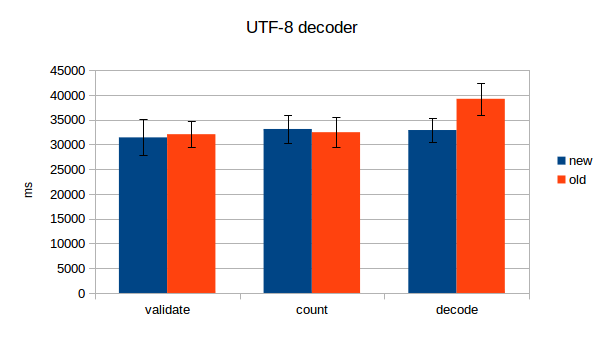
\includegraphics{utf8-decoder.png}

\section{UTF-8 string interning}
	This test was run with a different number of threads and concurrency factors.
	$new-N$ means the new hash table was configured with concurrency factor $N$.
	When running with multiple threads the work load was split evenly between all threads.

	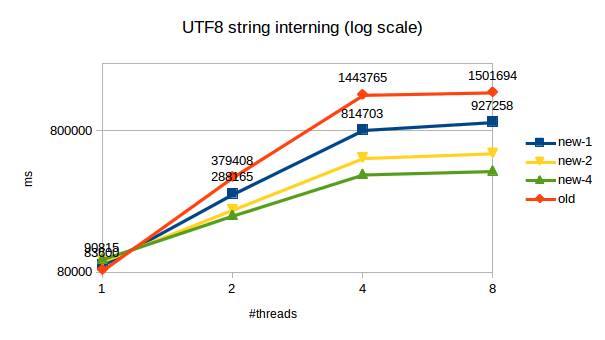
\includegraphics{utf8-intern-time.png}
	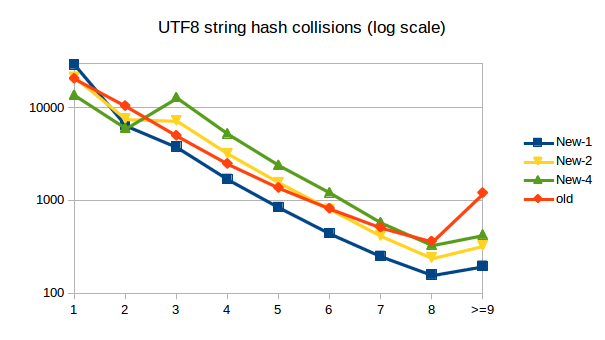
\includegraphics{utf8-intern-collisions.png}

	With only one thread the new intern table is actually slightly slower than the old one.
	But when more than one thread tries to access the table the new implementation is substantially faster.

	The average length of probes necessary to reach an item in the new table is actually longer than for the old
	one (2.68 vs 2.34), but the old table has far more items with an extremely high probe count.

	The entries in the new hashtable are evenly distributed across the $N$ buckets, each growing to the same size.
	And the number of entries varying less than $2\%$ regardless of concurrency factor.

\section{Java string interning}
	In this benchmark \java{java.lang.String} objects were created from already validated \cpp{Utf8String}s.
	This test was again run with a different number of threads and concurrency factors.

	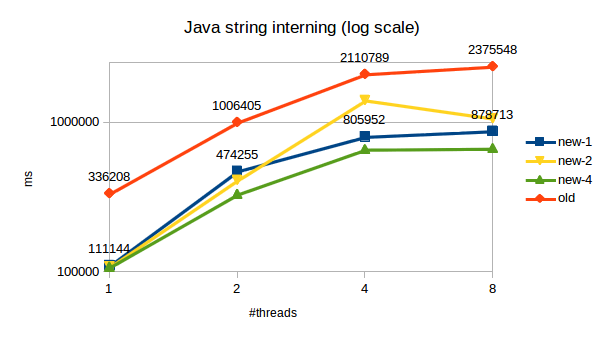
\includegraphics{jstr-intern-time.png}
	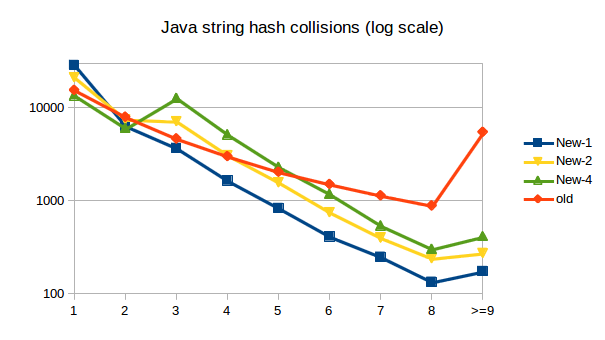
\includegraphics{jstr-intern-collisions.png}

	Using the stronger hash as the UTF-8 table and the lazy object creation have lead to a significant performance
	improvement for Java string interning.
	The new implementation now beating the old one in each test configuration.

\bibliographystyle{alpha}
\begin{thebibliography}{99}
	\bibitem{jvmutf8}
		The CONSTANT\_Utf8\_info Structure, §4.4.7 in the \emph{The Java® Virtual Machine Specification}.
		\url{http://docs.oracle.com/javase/specs/jvms/se7/html/jvms-4.html#jvms-4.4.7} (Oct 2013)
	\bibitem{utf8decoder}
		Bj\"{o}rn H\"{o}hrmann,
		Flexible and Economical UTF-8 Decoder.
		\url{http://bjoern.hoehrmann.de/utf-8/decoder/dfa/} (Oct 2013)
	\bibitem{pydict}
		Andrew Kuchling,
		Python's dictionary implementation: Being all things to all people.
		Beautiful Code, ISBN-13: 978-0596510046, O'Reilly Media, June 2007
	\bibitem{sparsehash}
		\emph{sparsehash - An extremely memory-efficient hash\_map implementation}
		\url{http://code.google.com/p/sparsehash/} (Oct 2013)
	\bibitem{ConcurrentHashMap}
		OpenJDK 1.7 ConcurrentHashMap
		\url{http://docs.oracle.com/javase/6/docs/api/java/util/concurrent/ConcurrentHashMap.html} (Oct 2013)
	\bibitem{DaCapo}
		DaCapo Benchmark Suite
		\url{http://www.dacapobench.org/} (Oct 2013)
	\bibitem{llvm}
		The Low Level Virtual Machine,
		http://llvm.org/
	\bibitem{bslassert}
		Build-specific, runtime-configurable assertion macros.
		Bloomberg Basic Standard Library,
		\url{http://bloomberg.github.io/bsl/group__bsls__assert.html} (Oct 2013)
	\bibitem{iwyu}
		Include What You Use,
		\url{http://code.google.com/p/include-what-you-use/} (Oct 2013)
	\bibitem{static_assert}
		Boost static\_assert
		\url{http://www.boost.org/doc/libs/1_54_0/doc/html/boost_staticassert.html} (Oct 2013)
\end{thebibliography}

\end{document}
